\chapter*{Preface}

This piece of notes covers one way of building a \textbf{static} website. It facilitates my live teaching sessions or my Web \& Git YouTube series.
\vspace{6mm}

We use \textbf{Pug.js} (sometimes abbreviated to Pug in this piece of notes) instead of HTML, \textbf{less} instead of CSS. And used gulp to translate the files back to HTML and CSS. The generated HTML files can be directly opened by the browser. We also included \textbf{Bootstrap} to make our static website responsive.
\vspace{6mm}

At the same time, we will be learning how to use \textbf{Git} and \textbf{command line tools}.

\section{Prerequisites}

Basic coding experience (e.g. variables, loops) in any programming languages (e.g. C++, Python) is expected. Knowing basic HTML and CSS would be helpful, but not necessary. 
% I would contrast HTML with Pug.js and CSS with less throughout the notes, if you have not learned HTML and CSS you could skip those sessions.

\section{Way to read the notes}

This piece of notes aims to fill the gaps of the online resources, and also acts as the bridge between different components of the project. It will not include every detail that you need to know, but I would try to include different online resources (documentations and YouTube tutorials) required in the form of hyperlinks along the way.
\vspace{6mm}

Hands on practice is also super important in programming, instead of revising this piece of notes over and over again, you will probably learn more if you make more websites on your own. :)
\vspace{6mm}

We start with installing the tools you need for this project. It is probably a bit complicated for most of you, but I reassure you that it is worth the time. It also tells you some basic tips to use the project. In order for you to have hands on experience with coding as soon as possible, \cref{sec:pug1} introduces the Pug.js syntax allowing you to edit the content of the web page. Then we go back to some boring\footnote{I guess the command line interface is not colourful is what makes it boring?} details in chapters 3-6. Then we go back to talk about styling in chapters 7-8. Finally, we will learn how to use variables in Pug.js in \cref{sec:pug2}. And we conclude by miscellaneous bits in \cref{sec:misc}.
\vspace{6mm}

However, feel free to move back and forth between chapters as long as you feel comfortable and fresh. 
\vspace{6mm}

I marked the less essential sections with \textit{Advanced} or \textit{Of less importance}. The whole of \cref{sec:git2} and \cref{sec:pug2} are labelled with \textit{Advanced}, while the whole of \cref{sec:misc} is labelled with \textit{Of less importance}. You can read the sections without the markings first, then those with \textit{Advanced}, then those with \textit{Of less importance}.

\section{Why?}

Why are we learning how to make a website? Why this particular framework? Why are we learning Git and command line tools at the same time?

I decided to delay answering these questions until the last chapter \cref{sec:rationale}, as it is easier to explain after you have learnt all the knowledge. For now, I would just give you some buzzwords in \cref{fig:objective} without explaining it. You can go ahead with the learning if you are motivated enough to do so. I wish you learn this also because you like it other than it being useful in some sense.
 
\begin{figure}[h]
\centering
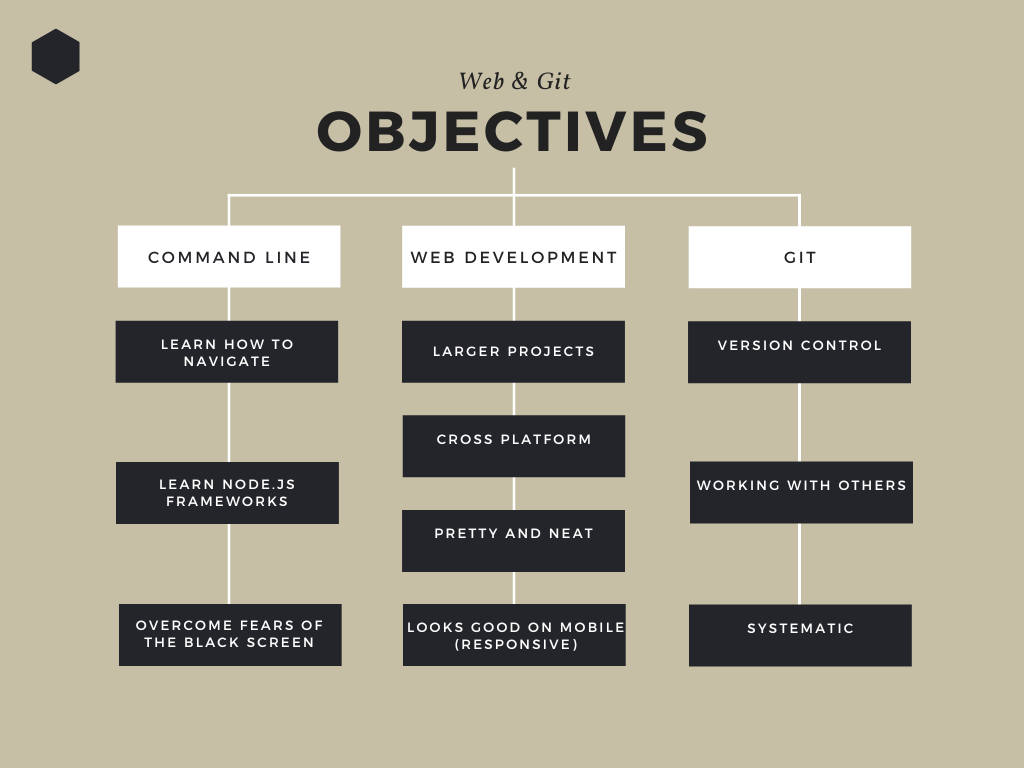
\includegraphics[width=15cm]{images/chn0-objectives.png}
\caption{Overview of the objectives for this course}
\label{fig:objective}
\end{figure}

\section{A word of warning}

This is just a draft, aiming to include everything in the shortest amount of time possible, so explanations and examples may be inadequate. If there are any errors in the notes feel free to contact me by email oscar.mui@univ.ox.ac.uk

\section{Linktree}

Useful links related to the notes.
\vspace{6mm}

Video series I made: \textit{(I have to admit they are not of the best quality, and the series is not finished yet)}

\url{https://www.youtube.com/playlist?list=PLjGmdnqrOKuYXiu7lgG5HW71jPEUd1XCm}
\vspace{6mm}

Example website:

\url{https://numbersarefun.netlify.app/}
\vspace{6mm}

Template for you to start from scratch:

\url{https://github.com/KidProf/static-web-sandbox}
\vspace{6mm}

Source code of the finished website:

\url{https://github.com/KidProf/numbersarefun-sample-temp}
\vspace{6mm}

Pug.js: 

\url{https://pugjs.org/}
\vspace{6mm}

Less: 

\url{https://lesscss.org/}
\vspace{6mm}

Bootstrap: 

\url{https://getbootstrap.com/}
\vspace{6mm}

